This Section firstly explains the steps of this system evaluation processes, aimed at measuring and comparing the performance (latency, in seconds, and throughput, in rows/second) of reading and writing Iceberg and Delta Lake tables on \gls{HopsFS}. Those experiments will be conducted respectively on the PyIceberg-based system, integrated in this thesis work, and on the Rust-based system, implemented in a related work \cite{manfrediReducingReadWrite2024}. Then, it presents the evaluation framework used by in this process.



%%%% EVALUATION PROCESS
\subsection{Evaluation process - RQ2 - Iceberg vs. Delta Lake}
\label{subsec:eval_process_iceberg_delta}
This evaluation process will follow a sequential approach described in Figure~\ref{fig:method_comparison}. Each step of this process is related to one of the \glspl{G}7--9 associated with the \gls{RQ}2 in Section \ref{sec:intro_goals}. The relationships between each process activity and \glspl{G} are here explained:
\begin{enumerate}
    \item \textbf{Analyze related work results}: this activity maps perfectly to \gls{G}7, analyzing the results coming from the related work took as input by this process.
    \item \textbf{Visualize results}: this activity maps perfectly to \gls{G}8. It takes as input also Iceberg experiments results (\gls{D}1-partial), visualizing thus the experiments' result according latenc and throughput. This activity generates \gls{D}2, the comparative experiments results complemented with tables and histograms, presented in Chapter \ref{ch:results_and_analysis}.
    \item \textbf{Analyze results}: this activity maps perfectly to \gls{G}9, analyzing and interpreting the results delivered in \gls{D}2. This activity contributes to \gls{D}3, generating the comparative analysis of the experiment results, presented in Chapter \ref{ch:results_and_analysis}.
\end{enumerate}
\begin{figure}[!ht]
    \begin{center}
    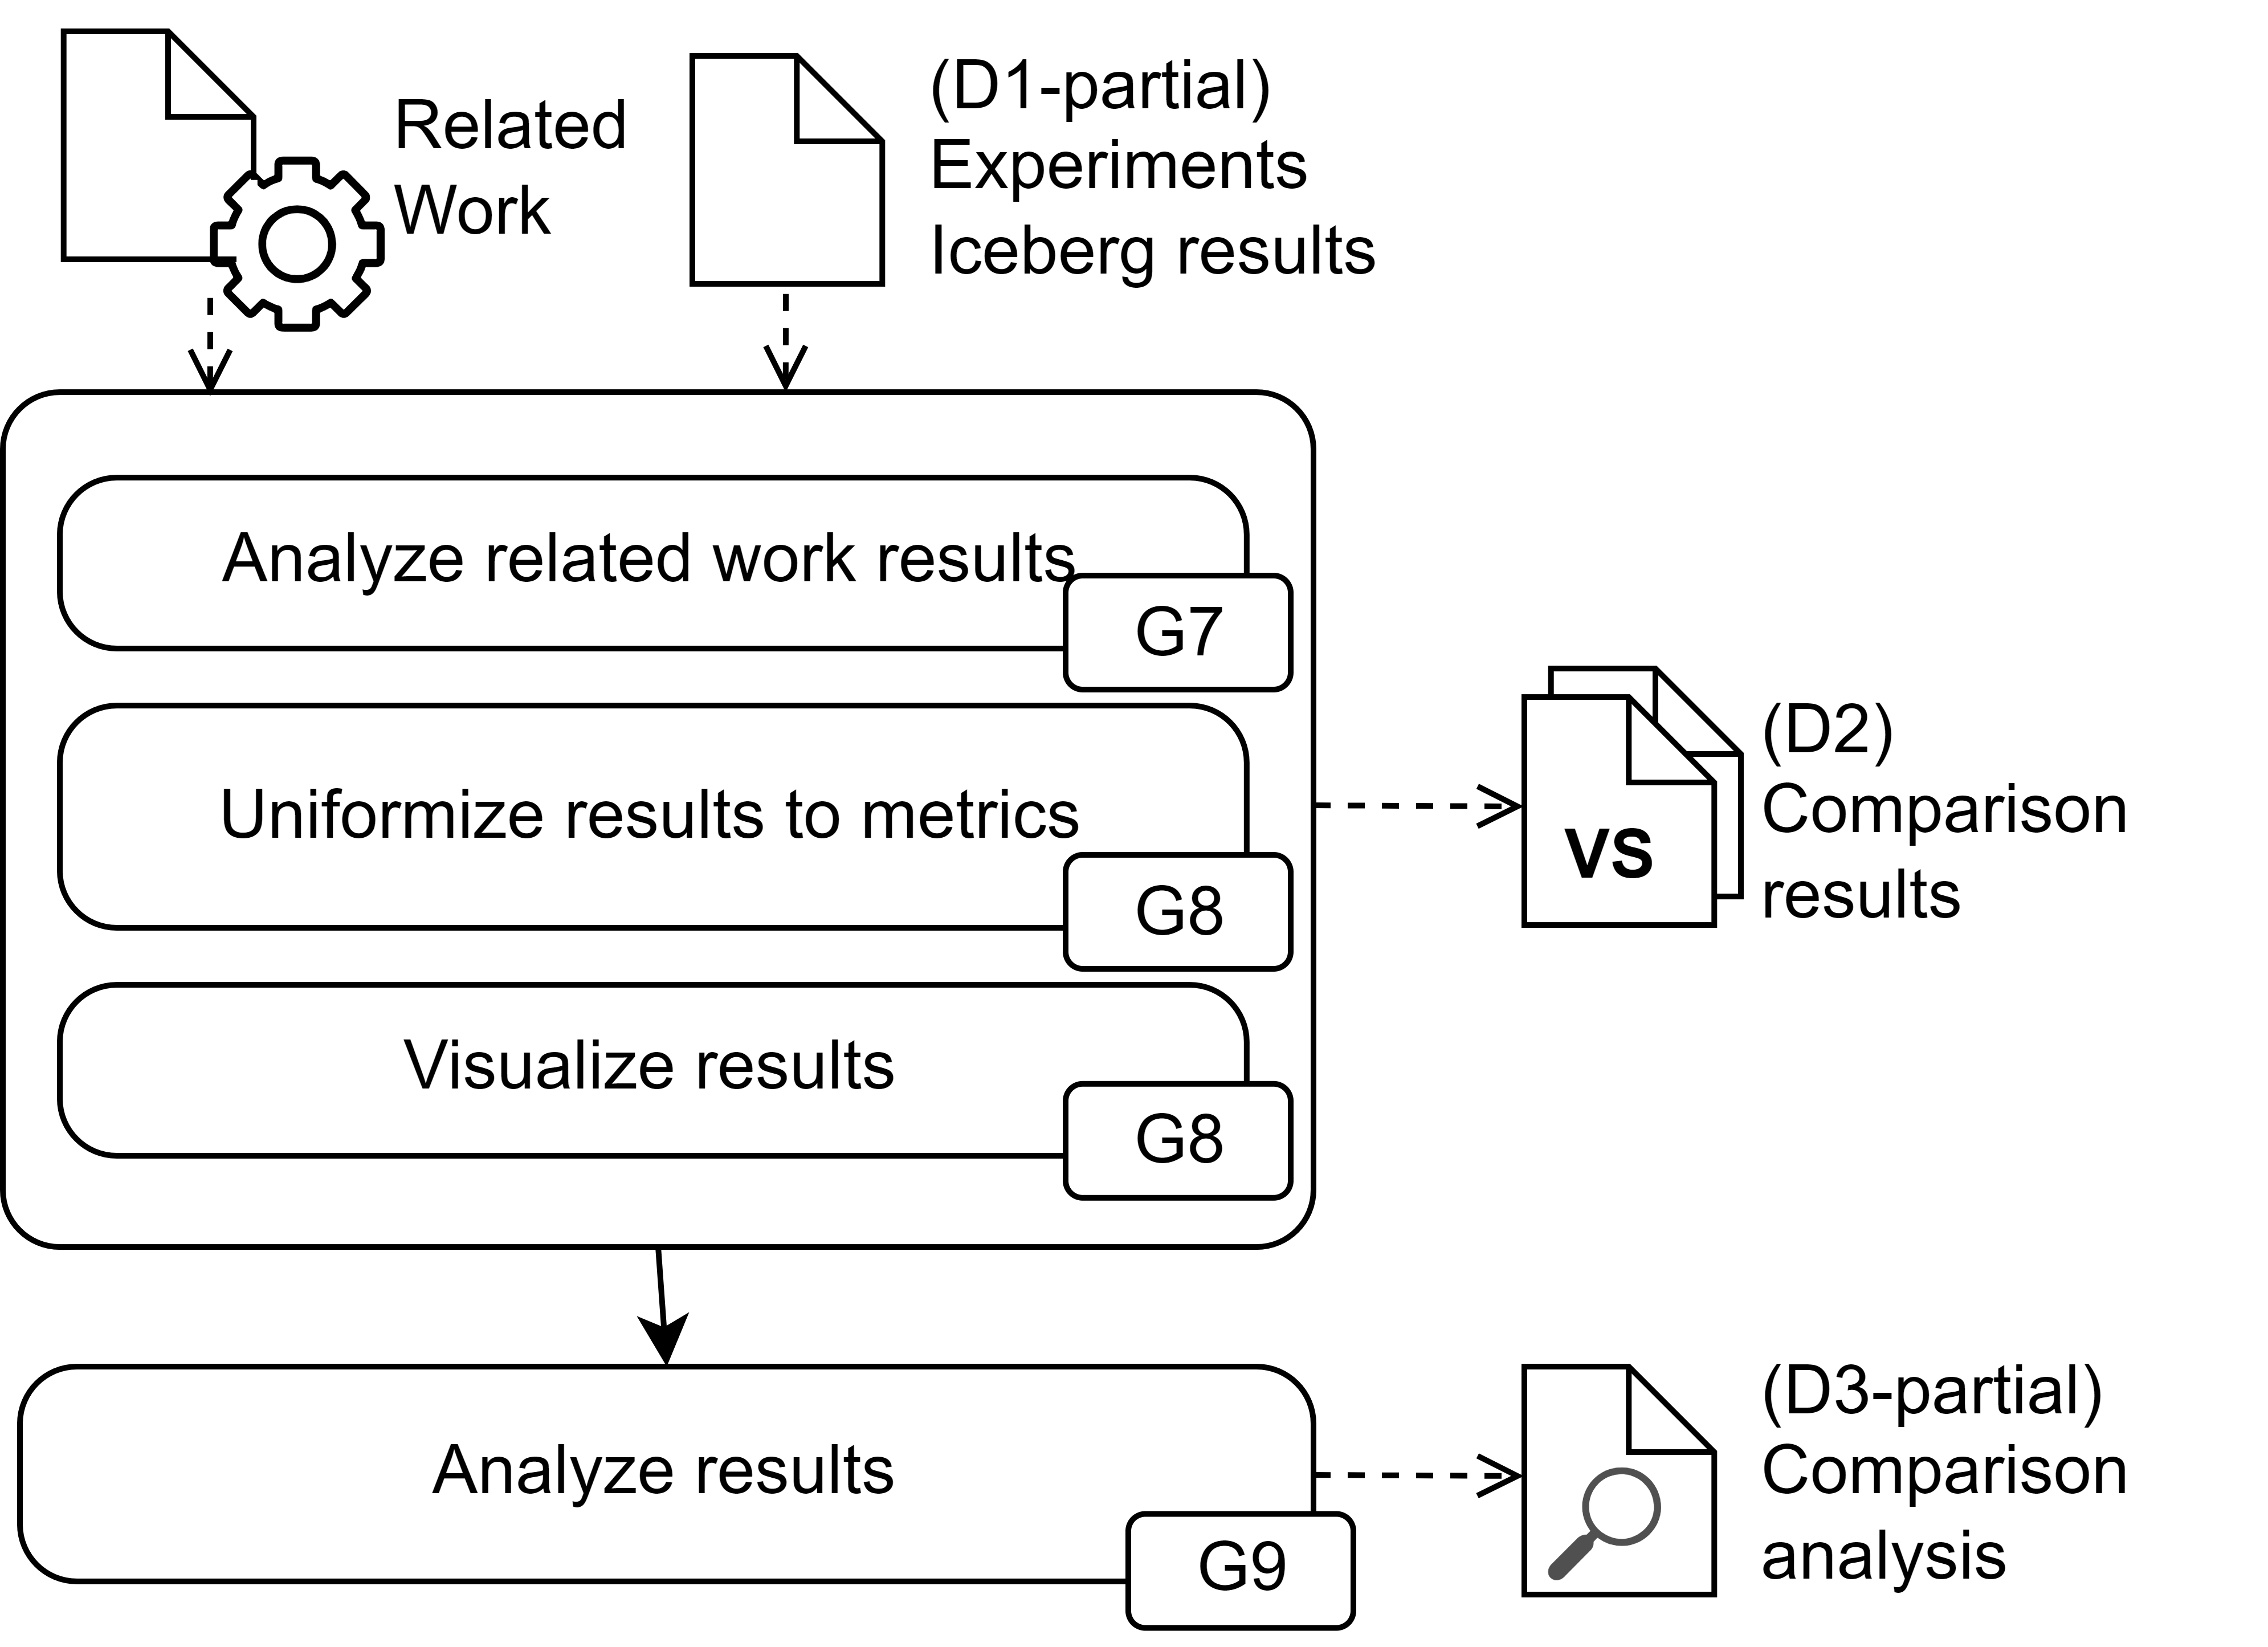
\includegraphics[width=0.7\textwidth]{figures/3-method/method_comp.png}
    \caption[System evaluation process - Iceberg vs. Delta Lake]{Diagram of the system evaluation process partially answering \gls{RQ}2. Each activity is associated to specific \gls{G}. The process produces two \glspl{D}, the comparative expertiments results (\gls{D}2) and a comparative results analysis (\gls{D}3-partial).}
    \label{fig:method_comparison}
    \end{center}
\end{figure}



%%%% EVALUATION FRAMEWORK
\subsection{Evaluation framework}
\label{subsec:method_eval_framework_iceberg_delta}

This system evaluation framework is similar to the system evaluation framework described in Section \ref{subsec:method_eval_framework_hudi_iceberg}, but will not focus on functional requirements, as they will be already assessed in previous Section, for Iceberg, and they have been already assessed in the related work, for Delta Lake. Thus, this evaluation framework will evaluate the different system on two key aspects:
\begin{enumerate}
    \item \textbf{Non-functional requirements}: Consistency and maintainability are mainly addressed during integration, while scalability is measured during the system evaluation experiments. The metric used for measuring this requirement is the throughput, as defined in \gls{RQ}2.
    \item \textbf{How does the PyIceberg pipeline compare to the Delta Lake pipeline?} this question answers directly \gls{RQ}2, measuring the throughput of the PyIceberg pipeline defined in Section \ref{subsec:experimental_design} and the Delta Lake pipeline \cite{manfrediReducingReadWrite2024}. Results are then compared using a visual approach.
\end{enumerate}


